\documentclass{beamer}[169]
\usepackage{wasysym}
\usepackage{tikz}
\usepackage{pgfplots}
\usepackage{epsf}
\usepackage{media9}
\usetikzlibrary{decorations.pathreplacing} % Acolades
\usetikzlibrary{arrows}
\usepackage{bm}
\usefonttheme{professionalfonts}
\usetheme{PaloAlto}
\usecolortheme{spruce}
\addtobeamertemplate{footline}
{%
   \usebeamercolor[fg]{author in sidebar}
   \vskip-1cm\hskip10pt
   %\insertpagenumber\,/\,\insertpresentationendpage\kern1em\vskip2pt%
   \insertframenumber\,/\,\inserttotalframenumber\kern1em\vskip2pt%
}

\title{Towards Hierarchical Explanation}
\author{Christiaan \and Hinrik \and Albert \and Anna}
\date{FACT-AI 2020}


\begin{document}

\frame{\titlepage}

\begin{frame}{Frame Title}
    \includemedia{img/tiny.mp4}
\end{frame}


\begin{frame}{Table of Contents}
\tableofcontents
\end{frame}



\section{Reproducing the prototype network}
\begin{frame}{Original paper}
    \begin{thebibliography}{99}
        \bibitem{deep}
        Li, Oscar and Liu, Hao and Chen, Chaofan and Rudin, Cynthia.
        \newblock Deep learning for case-based reasoning through prototypes: A neural network that explains its predictions.
        \newblock {\em Thirty-Second AAAI Conference on Artificial Intelligence}, 2018
    \end{thebibliography}
\end{frame}

\begin{frame}{Idea}
\begin{itemize}
    \item Broadly speaking, (convolutional) neural nets are not interpretable
    \item Instead of explaining with a new model after training, integrate explanations in training goal
    \item Learn a fixed amount of \alert{prototypes} which represent the entire dataset
    \item Model consists of an autoencoder an a prototype network...
\end{itemize}
\end{frame}

\begin{frame}{The prototype network}
\begin{figure}
    \makebox[\columnwidth][c]{
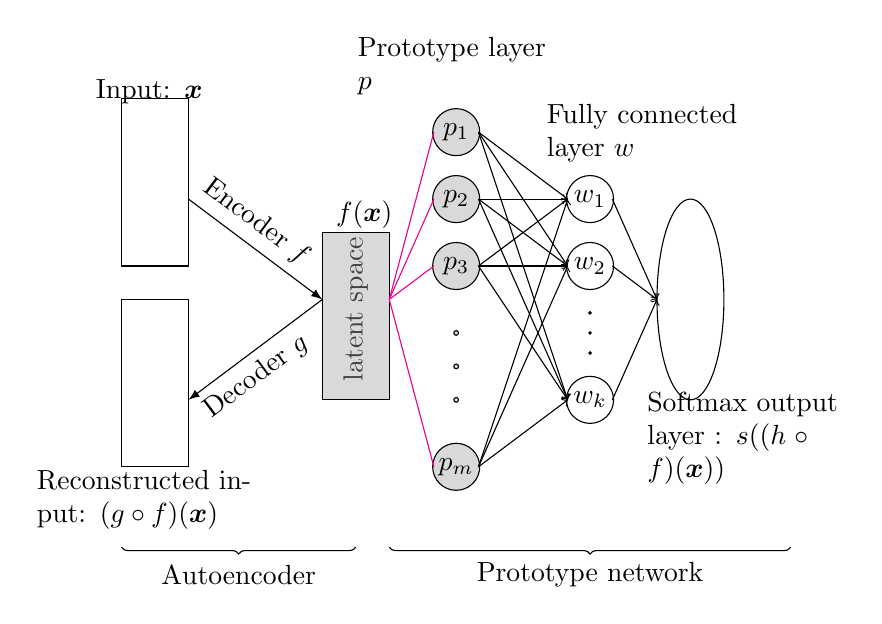
\begin{tikzpicture}[scale=0.85]
  \filldraw[fill=white, draw=black] (0,0) rectangle (1,2.5) ;
  \path (0,0) -- (1,2.5) node[midway, below,  yshift=-2.8em, text width=3cm] {Reconstructed input: $(g \circ f)(\bm{x})$ };
  \filldraw[fill=white, draw=black] (0,3) rectangle (1,5.5);
  \path (0,3) -- (1,5.5) node[midway, above, yshift=2.5em, text width=1.5cm] {Input: $\bm{x}$ };
;
\filldraw[fill=gray!30, draw=black] (3,1) rectangle (4,3.5);
\path (3,2) -- (4,4) node[midway, above, yshift=1em, xshift=0.75cm, text width=2cm]{ $f(\bm{x})$} node[color=darkgray,rotate=90,midway,xshift=-0.55cm] {latent space};
\path[-latex] (3, 2.5) edge node [xshift=-0.2cm, sloped, below] {Decoder $g$} (1,1) ;
\path[-latex] (1, 4) edge node [xshift=-0.2cm, sloped, above] {Encoder $f$} (3,2.5);
\coordinate (p1) at (5,0);
\coordinate (p2) at (5,2);
\coordinate (p3) at (5,3);
\coordinate (p4) at (5,4);
\coordinate (pn) at (5,5);
\coordinate (o1) at (7,1);
\coordinate (o2) at (7,2);
\coordinate (o3) at (7,3);
\coordinate (o4) at (7,4);
\filldraw[fill=gray!30, draw=black] (p1) circle (1em) node {$p_m$};
\filldraw[fill=gray!30, draw=black] (p2) circle (0.1em);
\filldraw[fill=gray!30, draw=black] (5,1.5) circle (0.1em);
\filldraw[fill=gray!30, draw=black] (5,1) circle (0.1em);
\filldraw[fill=gray!30, draw=black] (p3) circle (1em) node {$p_3$};
\filldraw[fill=gray!30, draw=black] (p4) circle (1em) node {$p_2$};
\filldraw[fill=gray!30, draw=black] (pn) circle (1em) node {$p_1$}  node[above, yshift=1em, text width=2.5cm] {Prototype layer $p$};
\filldraw[fill=white, draw=black] (o1) circle (1em) node {$w_k$};
\filldraw[fill=gray!30, draw=black] (7,2) circle (0.05em);
\filldraw[fill=gray!30, draw=black] (7,2-0.3) circle (0.05em);
\filldraw[fill=gray!30, draw=black] (7,2+0.3) circle (0.05em);
\filldraw[fill=white, draw=black] (o3) circle (1em) node {$w_2$};
\filldraw[fill=white, draw=black] (o4) circle (1em)node {$w_1$} node [above,yshift=1em, text width=2.5cm, xshift=2em] {Fully connected layer $w$};
 \foreach \i [evaluate=\i as \itext using int(\i)] in {0,3,4,5}
 {
    \path[color=magenta] (4.6666, \i) edge (4,2.5);
    \foreach \j [evaluate=\j as \itext using int(\j)]in {1,3,4}
    {
      \path[->] (5.333, \i) edge (6.666666666666, \j);
    }
  }
\filldraw[fill=white, draw=black] (8.5,2.5) ellipse (0.5 and 1.5) node[below,yshift=-3em, text width=2.5cm, xshift=2em] {Softmax output layer : $s((h\circ f)(\bm{x}))$};
  \foreach \j [evaluate=\j as \itext using int(\j)]in {1,3,4}
    {
      \path[->] (7.333, \j) edge (8, 2.5);
    }

    \draw [decorate,decoration={brace,mirror}] (0,-1.2) -- (3.5,-1.2) node[midway,yshift=-10pt]{Autoencoder};

    \draw [decorate,decoration={brace,mirror}] (4,-1.2) -- (10,-1.2) node[midway,yshift=-10pt]{Prototype network};
\end{tikzpicture}}

    \end{figure}
\end{frame}

\begin{frame}{Building the loss function}
\begin{block}{Loss function}
 \only<1>{Loss = Reconstruction error}
 \only<2>{Loss = Crossentropy loss + Reconstruction error}
 \only<3-5>{Loss = Crossentropy loss + Reconstruction error + Regularization terms}
 \only<1>{\[L((f,g)),D) = R(g \circ f, D)\]}
 \only<2>{\[ L((f,g,h),D) =E(h \circ f, D) +  R(g \circ f,D)\]}
 \only<3>{\[ L((f,g,h),D) =E(h \circ f, D) +  R(g \circ f,D) + R_1 + R_2\]}
 \only<4-5>{\[ L((f,g,h),D) = \lambda_{\text{class}}E(h \circ f, D) + \lambda_R R(g \circ f,D) + \lambda_1 R_1 + \lambda_2 R_2\]}
\end{block}
 \only<4->{ \begin{block}{Regularization terms for prototypes $\bm{p_1},\dots,\bm{p_m}$}
 \begin{align*}
     R_1(\bm{p_1}, \bm{p_2}, \dots, \bm{p_m}, D) = \frac{1}{m}\sum_{j=1}^m \min_{i\in [1,n]}||\bm{p}_j- f(\bm{x}_i)||^2_2 \\
     R_2(\bm{p_1}, \bm{p_2}, \dots, \bm{p_m}, D) = \frac{1}{{\color{blue}n}}\sum_{{\color{blue}i}=1}^{{\color{blue}n}} \min_{{\color{blue}j}\in [1,{\color{blue}m}]}||\bm{p}_j- f(\bm{x}_i)||^2_2
 \end{align*}
\end{block}}
\end{frame}


\begin{frame}{Reproducing results}
    \begin{itemize}
        \item MNIST digits
        \item Autoencoder with four convolutional layers
        \item Learning rate 0.0001, Epochs 1500 \pause
        \item Test accuracy: 98.879\% (Paper reports 99.22\%)
    \end{itemize}
\end{frame}

\begin{frame}{Learned prototypes}
\begin{itemize}
\item Original results:\\
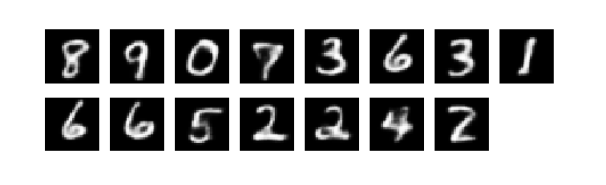
\includegraphics[scale=0.4]{img/originals.png}
\item Reproduced results:\\
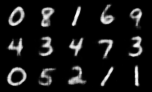
\includegraphics[scale=0.9]{img/reproduced42.png}
\end{itemize}
\end{frame}

\begin{frame}{However...}
\begin{itemize} 
\item Reproduced results with another seed:\\

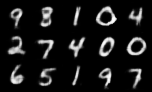
\includegraphics[scale=0.9]{img/reproduced9.png}

\item (Accuracy still 98.71\%)
\end{itemize}
\end{frame}


\section{The hierarchical prototype network}
\begin{frame}{The hierarchical idea}
\begin{itemize}
    \item Multiple prototypes of 1 class 
    \item Sometimes prototype network does not learn a prototype for each class
\end{itemize}
Solution: \alert{subprototypes}\pause
\begin{itemize}
    \item $ \text{Input example}\prec \text{Subprototype}\prec \text{Superprototype}$, \\
    Where $\prec$ means ``more specific than"
    \item \emph{More layers!}
    \item Allows network to learn each class in superprototype layer with $K$ superprototypes... \pause and more specific prototypes (eg. different types of 2's) in the subprototype layer.
\end{itemize}
\end{frame}

\begin{frame}{Two new loss terms}
\begin{block}{New loss term}
$L((f,g,h),D) = \lambda_{\text{class}}E(h \circ f, D) + \lambda_R R(g \circ f,D) + \lambda_1 R_1 + \lambda_2 R_2 + \lambda_3 R_3 + \lambda_4 R_4$
\end{block}
 \begin{align*}
R_1(\bm{p_1}, \dots, \bm{p_m}, D) &= \frac{1}{m}\sum_{j=1}^m \min_{i\in [1,n]}||\bm{p}_j- f(\bm{x}_i)||^2_2 \\
      R_2(\bm{p_1},  \dots, \bm{p_m}, D) &= \frac{1}{{\color{red}n}}\sum_{{\color{red}i}=1}^{{\color{red}n}} \min_{{\color{red}j}\in [1,{\color{red}m}]}||\bm{p}_j- f(\bm{x}_i)||^2_2\\
     R_3(\bm{P_1}, \dots, \bm{P_K}, \bm{p_1}, \dots, \bm{p_m}) &= \frac{1}{K}\sum_{k=1}^K \min_{j\in [1,m]}||\bm{P}_k- \bm{p}_j||^2_2 \\
    R_4(\bm{P_1}, \dots, \bm{P_K}, \bm{p_1}, \dots, \bm{p_m}) &= \frac{1}{{\color{blue}m}}\sum_{{\color{blue}j}=1}^{{\color{blue}m}} \min_{{\color{blue}k}\in [1,{\color{blue}K}]}||\bm{P}_k- \bm{p}_j||^2_2
 \end{align*}
\end{frame}

\begin{frame}{Our architecture}
    \makebox[\columnwidth][c]{
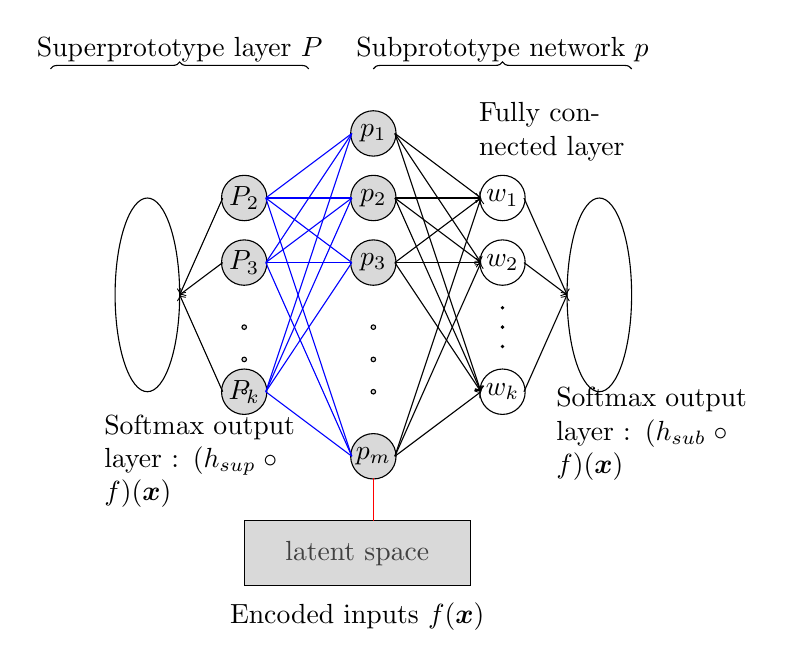
\begin{tikzpicture}[scale=0.82]
\coordinate (p1) at (1,0);
\coordinate (p2) at (1,2);
\coordinate (p3) at (1,3);
\coordinate (p4) at (1,4);
\coordinate (pn) at (1,5);
\coordinate (o1) at (3,1);
\coordinate (o2) at (3,2);
\coordinate (o3) at (3,3);
\coordinate (o4) at (3,4);

\coordinate (sp1) at (-1,1);
\coordinate (sp2) at (-1,2);
\coordinate (sp3) at (-1,3);
\coordinate (sp4) at (-1,4);
\coordinate (spn) at (-1,5);
\coordinate (so1) at (-3,1);
\coordinate (so2) at (-3,2);
\coordinate (so3) at (-3,3);
\coordinate (so4) at (-3,4);
% SUPER
\filldraw[fill=gray!30, draw=black] (sp1) circle (1em) node {$P_k$};
\filldraw[fill=gray!30, draw=black] (sp2) circle (0.1em);
\filldraw[fill=gray!30, draw=black] (-1,1.5) circle (0.1em);
\filldraw[fill=gray!30, draw=black] (-1,1) circle (0.1em);
\filldraw[fill=gray!30, draw=black] (sp3) circle (1em) node {$P_3$};
\filldraw[fill=gray!30, draw=black] (sp4) circle (1em) node {$P_2$};
%\filldraw[fill=gray!30, draw=black] (spn) circle (1em) node {$s_1$}  node[above, yshift=1em, text width=3cm, xshift=1em] {Superprototype layer};
\filldraw[fill=white, draw=black] (-2.5,2.5) ellipse (0.5 and 1.5) node[below,yshift=-4em, text width=2.5cm, xshift=2em] {Softmax output layer : $(h_{\text{sup}}\circ f)(\bm{x})$};
\foreach \j [evaluate=\j as \itext using int(\j)]in {1,3,4}
{
  \path[->] (-1.333, \j) edge (-2, 2.5);
}
\filldraw[fill=gray!30, draw=black] (-1,-1) rectangle (2.5,-2) node[color=darkgray,midway] {latent space} node[color=black, midway, below, yshift=-0.5cm] {Encoded inputs $f(\bm{x})$};

% SUB
\filldraw[fill=gray!30, draw=black] (p1) circle (1em) node {$p_m$};
\filldraw[fill=gray!30, draw=black] (p2) circle (0.1em);
\filldraw[fill=gray!30, draw=black] (1,1.5) circle (0.1em);
\filldraw[fill=gray!30, draw=black] (1,1) circle (0.1em);
\filldraw[fill=gray!30, draw=black] (p3) circle (1em) node {$p_3$};
\filldraw[fill=gray!30, draw=black] (p4) circle (1em) node {$p_2$};
\filldraw[fill=gray!30, draw=black] (pn) circle (1em) node {$p_1$};
\filldraw[fill=white, draw=black] (o1) circle (1em) node {$w_k$};
\filldraw[fill=gray!30, draw=black] (3,2) circle (0.05em);
\filldraw[fill=gray!30, draw=black] (3,2-0.3) circle (0.05em);
\filldraw[fill=gray!30, draw=black] (3,2+0.3) circle (0.05em);
\filldraw[fill=white, draw=black] (o3) circle (1em) node {$w_2$};
\filldraw[fill=white, draw=black] (o4) circle (1em)node {$w_1$} node [above,yshift=1em, text width=2cm, xshift=2em] {Fully connected layer};
 \foreach \i [evaluate=\i as \itext using int(\i)] in {0,3,4,5}
 {
    \foreach \j [evaluate=\j as \itext using int(\j)]in {1,3,4}
    {
      \path[->] (1.333, \i) edge (2.666666666666, \j);
    }
  }
\filldraw[fill=white, draw=black] (4.5,2.5) ellipse (0.5 and 1.5) node[below,yshift=-3em, text width=2.5cm, xshift=2em] {Softmax output layer : $(h_{\text{sub}}\circ f)(\bm{x})$};
  \foreach \j [evaluate=\j as \itext using int(\j)]in {1,3,4}
    {
      \path[->] (3.333, \j) edge (4, 2.5);
    }
 \draw [decorate,decoration={brace}] (1,6) -- (5,6) node[midway,yshift=0.25cm]{Subprototype network $p$};
 \draw [decorate,decoration={brace}] (-4,6) -- (0,6) node[midway,yshift=0.25cm]{Superprototype layer $P$};
 
 \draw [color=red] (1,-1) edge (1,-0.33); 
  \foreach \i [evaluate=\i as \itext using int(\i)] in {0,3,4,5}
 {
    \foreach \j [evaluate=\j as \itext using int(\j)]in {1,3,4}
    {
      \draw[color=blue] (0.6666, \i) edge (-0.666, \j);
    }
  }
\end{tikzpicture}}

\end{frame}

\begin{frame}{Our architecture}
\begin{itemize}
    \item 
\end{itemize}
\end{frame}

\section{Hierarchical results}
\begin{frame}{Results}
\begin{itemize}
    \item Accuracy for superprototype classifier: 98.86\% %5999999999997 
    \item Accuracy for subprototype classifier:  99.02\%
\end{itemize}
\end{frame}
\begin{frame}{Superprototypes and subprototypes}
\begin{itemize}
 \item $K$ Superprototypes:\\   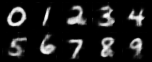
\includegraphics[scale=0.9]{img/hier42prot1499.png}

 \item $m$ Subprototypes: \\   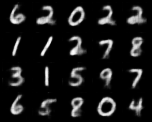
\includegraphics[scale=0.9]{img/hier42subprot1499.png}
\end{itemize}
\end{frame}

\section{Discussion}
\begin{frame}{What does this mean for transparency? }
    \begin{itemize}
        \item Something something interpretability
        \item Model interclass and intraclass variation
        \item Something something bias
    \end{itemize}
\end{frame}

\begin{frame}[plain]

\advance\textwidth2cm
\hsize\textwidth
\columnwidth\textwidth
\huge
\alert{Thank you for your attention}\pause \\
Any questions?
\end{frame}



\end{document}